% 2010 年浙江卷文科第 20 题：平行四边形 ABCD 沿 DE 翻折成 △A'DE（透视示意）。
% 来源 PDF：普通高考/2010/2010浙江文.pdf，SHA-256 a73e22ea405697775b2d5cd82532fcffad0f506b849d9f199265b4297b8a754b。
% 原页：第 2 页（A3 三栏）第 1 栏下部，书页码 642。
% 重绘依据：照原页透视，A 左下、E 在 AB 中点、B 右下、D 左、C 右、A' 在上；
%   F 为 A'C 中点、M 为 DE 中点。原页虚线为 D–C 与 M–F，其余（AE、EB、AD、DE、
%   A'D、A'E、A'C、BC、BF）均为实线。
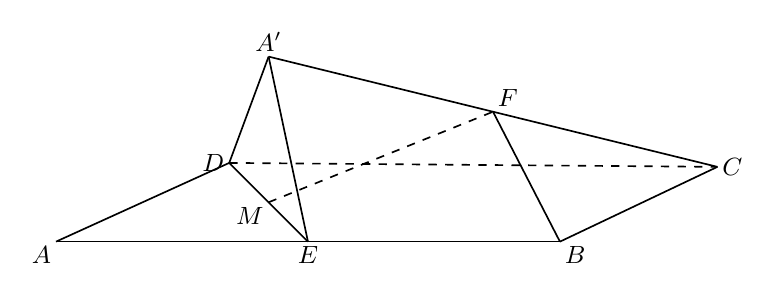
\begin{tikzpicture}[scale=1.0, semithick, every node/.style={inner sep=1.5pt, font=\small}]
  \coordinate (A)  at (0,0);
  \coordinate (E)  at (3.2,0);
  \coordinate (B)  at (6.4,0);
  \coordinate (D)  at (2.2,1.0);
  \coordinate (C)  at (8.4,0.95);
  \coordinate (Ap) at (2.7,2.35);
  \coordinate (F)  at (5.55,1.65);
  \coordinate (M)  at (2.7,0.5);

  % 底面与侧面
  \draw (A) -- (E) -- (B);
  \draw (A) -- (D);
  \draw (D) -- (E);
  \draw (B) -- (C);

  % 翻折后的三角形
  \draw (Ap) -- (D);
  \draw (Ap) -- (E);
  \draw (Ap) -- (C);
  \draw (B) -- (F);

  % 虚线：被遮挡的 D–C 与线段 M–F
  \draw[dashed] (D) -- (C);
  \draw[dashed] (M) -- (F);

  \node[above] at (Ap) {$A'$};
  \node[above right] at (F) {$F$};
  \node[below left] at (A) {$A$};
  \node[below] at (E) {$E$};
  \node[below right] at (B) {$B$};
  \node[left] at (D) {$D$};
  \node[right] at (C) {$C$};
  \node[below left] at (M) {$M$};
\end{tikzpicture}
